%===============================================================================
% $Id: ifacconf.tex 19 2011-10-27 09:32:13Z jpuente $  
% Template for IFAC meeting papers
% Copyright (c) 2007-2008 International Federation of Automatic Control
%===============================================================================

\documentclass[12pt]{ifacconf}
\usepackage{mathptmx}
\usepackage{graphicx}      % include this line if your document contains figures
\usepackage{natbib}        % required for bibliography

\usepackage[letterpaper,left=1truein,top=1truein,right=1truein,bottom=1truein,nohead]{geometry}
%\setlength\topmargin{0pt}
%\addtolength\topmargin{-\headheight}
%\addtolength\topmargin{-\headsep}
%\setlength\oddsidemargin{0pt}
%\setlength\textwidth{\paperwidth}
%\addtolength\textwidth{-2in}
%\setlength\textheight{\paperheight}
%\addtolength\textheight{-2in}
%\usepackage{layout}

%===============================================================================
\begin{document}

\begin{frontmatter}


\title{Agent-Based Modeling of Cell Pattering with Syn-Notch Signaling} 
% Title, preferably not more than 10 words.



\author[First]{Roberts C. Thomas} 


\address[First]{Cornell University, 
   Ithaca, NY 14850 USA (e-mail: tcr55@cornell.edu).}


\begin{abstract}      % Abstract of not more than 250 words.
\begin{bfseries}
 
 
{\large Background:}  Agent modeling is a powerful tool for observing the emergent phenomenon of cell pattering during development. Agent-based modeling allows for observation of the effects signaling circuits have on spatial cell pattering. With the wide use of Notch-Delta signaling in cell development and in engineered cell signaling circuits, agent-based modeling is an important tool in the ability to explore potential circuits in silico for observations that can improve experiment design and drive exploration of the parameters that shape cell patterns.
 
{\large Results:}  In this paper the Drosophila fly model developed by Reynolds etc Al. was extended to capture cell pattering features that arise in synthetic notch delta circuits in cells as shown in Todo etc Al. The key circuits tested were the Two and Three circuit design from Todo, Single genotype two layer. An extended circuit was tested which embedded a secondary syn-notch circuit into the singe genotype two layer to observe changes in the emergent phenomenon seen by Reynolds.
 
{\large Conclusion:} The extended model developed from the base work from Reynolds etc Al was able to both verify single genotype two layer, and was able to capture key features of the circuits tested in Todo etc al when under diffusion constraints. The addition of cell mobility extended the capabilities of the original model to test pattering under non-fixed cell populations.
\end{bfseries}
\end{abstract}

\begin{keyword}
Delta, Notch, SynNotch, Agent, Modeling
\end{keyword}

\end{frontmatter}
%===============================================================================

\section{Introduction}
Agent based modeling is a field of computer based modeling that uses a bottom up approach to designing a system.. \cite{Bon:02}. Agents, as they are called in agent based modeling, are the small sub units of the model that operate under a supplied logic. each agent is autonomous and acts independently from other agents. The logic of the agents however does allow for interactions to be modeled between agents. For example \citet{DB:08} leverages the use of agent based modeling to model crowd behavior, where the motion, direction, and speed of the cars, or agents, depend on the number of other cars the agent senses around it. This develops a model then of traffic \cite{DB:08}. Agent based models have been extended further than simple crowd behavior into more complex interations, namely health accplications or modeling the economy. \cite{FE:09}.

Cellular organization occurs when many cells signal among themselves, sensing their environment and taking cues from neighboring cells that end in the determination of the fate of the cell. \cite{KI:93}. In the context of cellular organization, particularly the pattering that arises, agent based methods are a tool that has appeared as a means of further probing the features of the patterning that arise from parameters of individual cells. Reynolds etc al took this approach in their \emph{Systems Biology} paper where they sought to model the development and subsequent patterning of Drosophilla cells in the agent based modeling program \emph{NetLogo} (\cite{RAB:19}). Portions of the development of drosophilla cell formation create unique patterns between two cell lines, neurons and the endothelial cells, where the neurons become surrounded by endothelial cells. This pattern leads to the formation of the eye disk in the flies. \cite{KI:93}. Reynolds termed these regions "Rosettes" and modleded them as a neuron cell surrounded by six endothelial cells. The signaling that was driving the formation of these patterns is called Delta-Notch and accurate understanding of the path drives robust model developemnt. 

Therfore it is important in the modeling to understand the signaling pathway. In \emph{Drosophilla} cell development the pathway called \emph{Notch-Delta} as mentioned before is responsible for cell fate determination. \cite{LN:04},  \cite{ATN:95} . Notch-Delta signaling occurs when cells express membrane bound receptors called Notch, and membrane bound ligands called Delta. The pathway has been extensively studied and figure 1 outlines the scheme by which cellular signaling occurs. Delta ligans bind to the extracellular region of Notch receptors on neighboring cells, which triggers a cleavage site to be exposed and the Notch receptor undergoes a transformation. Notch is composed of two regions, an external receptor region that binds to delta, and an internal region that contains the portion that will seek out the nucleus and signal or inhibit cellular fate. The two regions are cleaved when Delta binds to the extracellular region of notch and the internal Notch is trafficked to the nucleus. A key feature of Notch-Delta signaling is the inhibitory nature of Notch on delta, where more Notch production leads to a reduction in Delta production. This allows the system to become unbalanced, and one cell will eventually lead to over expression of Notch and assume one fate, while the other cell will produce delta and assume a different cell fate. this contact inhibition is what leads to the "rosette" patterns observed by Kooh and modled by Reynolds. 

This pathway is key to development of cells in \emph{Drosophilla} from \cite{KI:93}, however it has also been a key tool in the engineering of cell fate and signaling to further understand how cells organize during and after signaling events. Called \emph{Syn-Notch}, \cite{TP:18} used alterations of the standard Delta-Notch pathway and developed cell lines that would only express delta, only express Notch, or would express both and used these engineered cell lines to form unique patterns between cells. For example, in the \emph{ Two Later Circuit} Todo creates two genotypes of cells, one expressing delta and one expressing Notch with a florescent signal and a gene for cadherin production when notch is cleaved (\cite{TP:18}). The syn-notch signaling causes cell line A to activate cell line B's ability to express fluorescence and produce cadherin, where after the initial signaling the B cells begin sticking together due to the cadherin.  The result Todo shows are layers of cell formation, or islands of b cells surrounded by A cells (\cite{TP:18}). 

Extension of the Reynolds model to the Todo paper holds the potential to verify in silico the results of the Todo and Reynolds paper, but more importantly allows for the adaptation of the model to fit Delta-Notch signaling circuits outside of the \emph{Drosophilla} single genotype circuit Reynolds initially proposed. The new models generated in this paper were able to capture several key features of the cell patterns observed by Todo and verified the use and results of Reynolds model methodology towards extra Delta-Notch circuits. This is particularly useful when cell motion was factored into the Two layer model, as this feature is important in a dynamic system. The model could recapture many key feactures of the pattern and the results from the cell motion addition in Two layer exposes future new applications and modifications to the circuits considered here.

\begin{figure}
\begin{center}
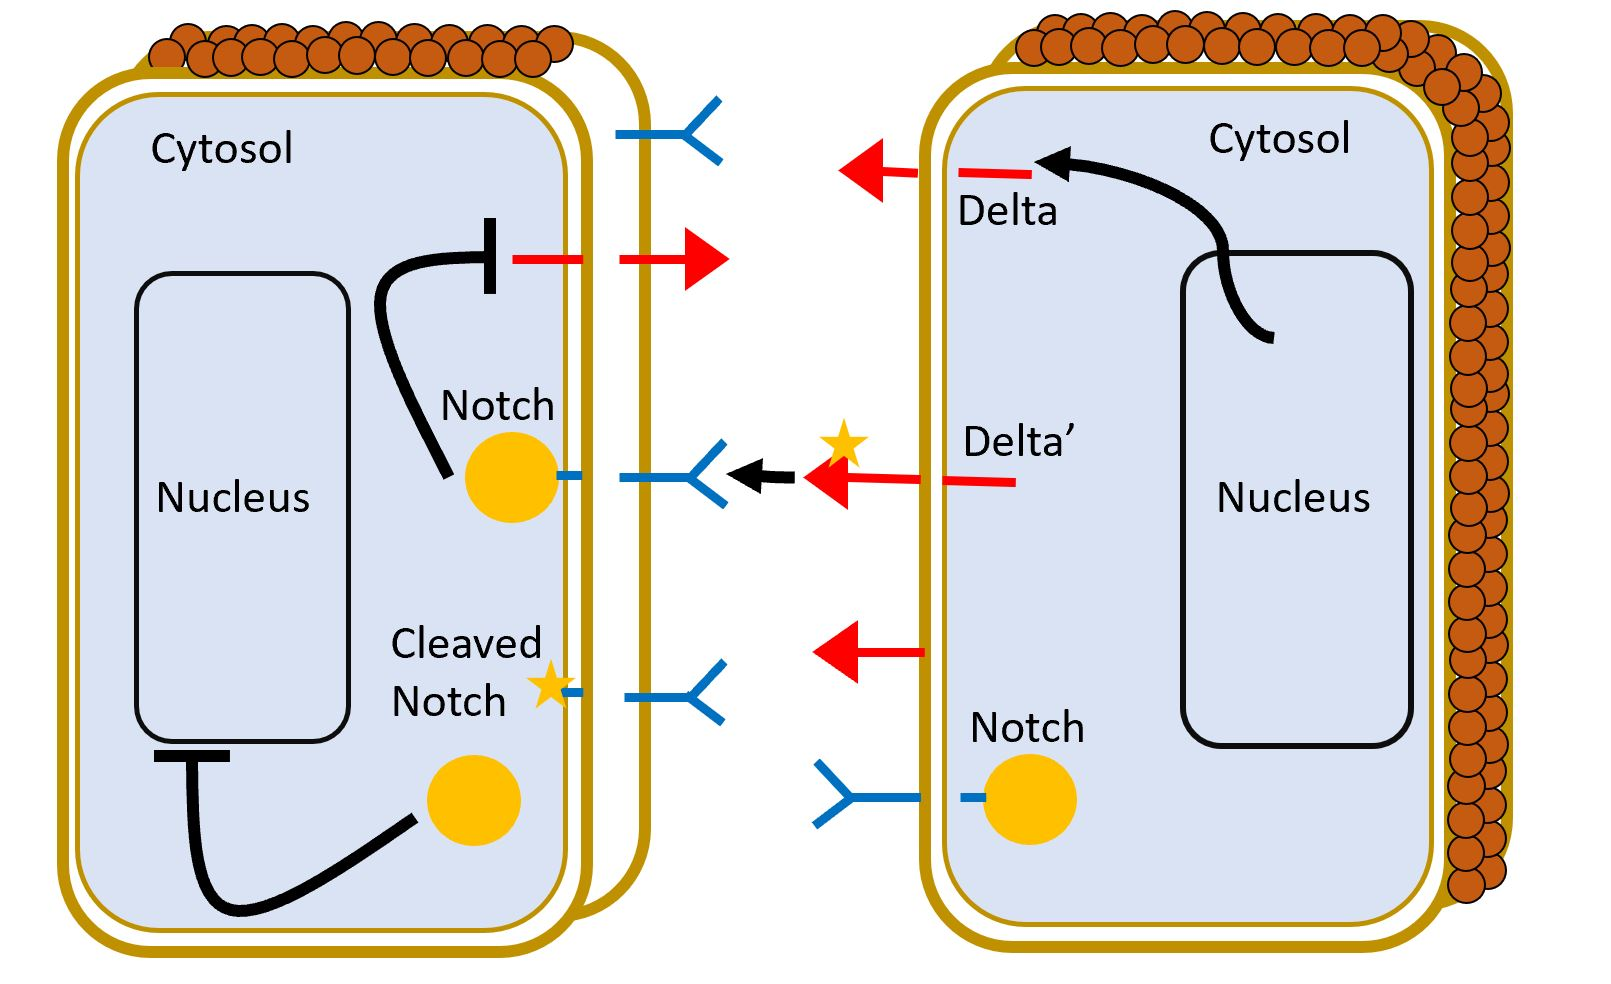
\includegraphics[width=8.4cm]{Overview_of_Delta_Notch}    % The printed column width is 8.4 cm.
\caption{Overview of the Delta-Notch Signaling pathway: Nucleus of the cells produce Delta and Notch membrane proteins. Delta protein is modeled to enter an activated Delta prime state according to Reynolds etc al. Delta Reacts with Notch, which leads to the cleavage of the internal region of Notch, which will then be known as Cleaved Notch or Nuclear Notch inside the nucleus in this paper. Subsequent repression or activation of cellular genes occurs once Nuclear Notch reaches the nucleus. Notch also represses expression and thus the activity of surrounding Delta membrane proteins, and eventual equilibrium will result in one cell over expressing Notch and the other cell expressing Delta. This leads to an oscillation of cell expression until the equilibrium is settled and cell fates are determined. } 
\label{fig:bifurcation}
\end{center}
\end{figure}


 %\texttt{ifacconf}
%\footnote{
%This is the default for the provided class file.}




\section{Methodology}

The base for the agent based model was the \emph{Drosphilla} cell model developed by \cite{RAB:19}. The modifications to the base model builds upon the Delta-Notch signaling using the Syn-Notch circuits developed by \cite{TP:18} as an inspiration. The circuits tested are \emph{Two Genotype Two Layer}, \emph{Two Genotype Three Layer}, \emph{One Genotype Contact Inhibition}, \emph{One Genotype Contact Inhibition Two Syn-Notch} (\cite{TP:18}).  Two Layer was further modified to include the motion of the cells to introduce cell mobility into the model and allow for expression of cadherin to be modeled. A longer detailed explination of the features and operation of the models is provided in Appendix A and reiterated in the Github source readme. 

The basic model without modifications operates using agents to model the following components of Notch-Delta signaling: Neucleus of the cell, the Delta and Notch proteins, Cleaved Notch protein, Nuclear Cleaved Notch protein, Delta Prime, and membrane bound Delta and Notch proteins. Shown in figure 1 is the basic signaling pathway that was modeled. Retaining the naming convention established by \cite{RAB:19} Nucleus agents are called Nucleus and are told to produce Notch and Delta agents depending on the circuit, of which modifications for each circuit will be discussed in their following subsections. These Notch and Delta agents are given a randomized direction and told to "diffuse" out in a straight line towards the modeled cell membrane. The cell membrane is modeled as Lipid agents and are formed in rows of 6 in a hexagonal shape with the Nucleus-breed centered at the middle (\cite{RAB:19}). As Notch and Delta agents approach the Lipid agents Reynolds model asks the Lipid agents and the Notch and Delta agents to come within 1 distance unit of each other. When the Notch and Delta agents have gotten close enough they will transition into Membrane Notch and Delta agents and their movement is constrained to move only laterally along Lipid agents, i.e 2 D motion along the length of the lipids. After a provided parameter time for transition Lipid Delta agents will transform into active Delta Prime agents and will continue to move along the hexagonal membrane lipids. the activity of the signaling occurs when a Notch membrane agent on cell A is directly opposite from a Delta membrane agent on cell B. Cleaved Notch is created as the "cleavage" event. The Cleaved notch is told to remain inside the cell just behind the membrane, where then the Cleaved notch agent will move towards the nucleus. Once the agent reaches a parameter set distance (for visualization) from the nucleus it converts into a nuclear Cleaved notch agent and its total motion is halted. (\cite{RAB:19})

Behavior of the expression of the cell is then added depending on the fate that levels of Nuclear Cleaved Notch agent determine according to circuit framework from \cite{TP:18} . Key modifications present in every model was the flourescence that \cite{TP:18} used to identify cell lines. The color is mapped to levels, or lack theroef, of cleaved nuclear Notch and color coding was kept consistent with \cite{TP:18} experimental tagging.

\subsection{Two Genotype -  Two Layer Circuit}

The Two genotype - Two layer circuit is modeled based of of the Todo etc al. circuit design seen in figure 2A. Cell line agents were modeled by removing the abiltiy to produce both Delta and Notch proteins at the same time, instead producing only Delta or only Notch. First type A cells are chosen at random using NetLogo's random number selector and these cells will produce Delta, all other cells will produce Notch. The cells that produce delta agents will turn blue to mimic florescence. Adjacent B cells that have membranes that neighbor the A cells will be signaled by them. When a Notch cleavage occurs in the B cells, Cleaved nuclear Notch is eventually formed, and when it passes a threshold the cell will turn green indicating the Delta from the A cells has signaled activity in the B cells. In addition to the modeled fluorescence, the B cells are given the ability to express cadherin according to the circuit. 

In addition, the Two genotype Two layer circuit has added mobility to covert the static lattice used in the Reynolds paper into a diffusing medium of cells. A random number generator again chooses random cells, however now it tells each chosen cell to move in a random direction. The goal is to mimic primitive diffusion of cells among the medium. Cells are constructed of the nucelus, lipid, and any membrane bound Notch or Delta and Cleaved Notch, and the diffusing Notch and Delta components. A bias towards the right of the simulation was added to improve mixing of the cells, as limitations in speed and computing intensity rose signinficantly under the addition of movement. The movemnt if allowd simple diffusion would stall out before good mixing would occur. Good mixing is considered as A cells having the oppurtuinity to signal more than their starting agecent neighbors to differentiate it from the static lattice model.

\subsection{Two Genotype - Three Layer Circuit}

The Three layer circuit with Two genotype is modeled based on the circuit design seen in figure figure 2B from \cite{TP:18}. Cell line agents in the Two layer had either Notch or Delta functionality to denote difference in genotype, however in Three layer circuit modeling the cells retain full functionality of the entire Notch-Delta signaling. The modifications to create the circuit are that cell line A expresses Delta 1 and Notch 2 while Cell line b expresses Delta 2 and Notch 1. Delta 2 is not compatible with Notch 1 and likewise for Notch 2 and Delta 1. This creates a feedback after the initial Notch-Delta signal event where A cell's Delta 1 activate B cell's Notch 1, leading to cell fate C and activating the expression of both the green fluorescence and the expression of Delta 2. Delta 2 feeds back on the A cells that activated the B cell and binds the Notch 2 on the A cells surface. This leads to the third D cell fate which is modeled to flouresce pink to be consistent with Todo etc al circuit design. Mobility was not modeled in this circuit design however geometry was constrained to mimic the layering found in the experimental results from \cite{TP:18}. 


\subsection{Single Genotype - Single Notch Two Layer Circuit}

Single Two layer circuit is identical to the model the Reynolds paper developed, where the circuit desing is seen in figure 3A. In single notch circuits both cells are of the same genotype, expressing both Notch and Delta. The result is a "tug of war" between the cells as differences in the rate of Notch and Delta production and location on the membrane lead to eventual imbalances which settles to eventually developing the two cell fates. One cell overexpressing Notch forces the cell fate of the other to express delta in excess, and eventually the fates are reinforced as notch inhibits delta expression and vice versa. random diffusion was modeled as discussed above to allow for these imbalances to arise, and the addition of the flouresence code to the model allowed for a direct comparison between Todo results for Two layer Single notch before cadherin agglomeration and Reynolds \emph{Drosophilla} cell sheet layout. The experiments were therefore verified as a control to ensure Reynolds code could accurately represent Todo's results before any major circuit modifications. This also acts as the control to check that the added florescence idicators accurately represented the cells. 

\subsection{Single Genotype - Double Notch Three Layer Circuit}

Single Genotype Three layer is an extension from the Reynolds \emph{Drosophilla} model taking inspiration from Todo's three layer circuit design, a layout and overview of the circuit is in figure 3B. Initially cells are modeled to behave identically to a Two layer Single genotype contact inhibition model. After an accumulation of Cleaved Notch from the Delta-Notch signaling passes a set parameter called "threshold" the cell's begin expressing a second Delta-Notch pathway. The second Delta-Notch pathway behaves identically to the firts Delta-Notch path, with the ability to tune the secondary pathways parameters.The fates of the cell were determined based on three fates: no Cleaved notch is a blue neuron cell, only Cleaved notch from the first pathway is a endothelial cell as before, and presence of both Cleaved notch from the first pathway and Cleaved notch from the second pathway indicate a third unnamed line of new type 2 endothelial cells. The intention in this addition is to observe whether additional Delta-Notch pathways lead to collapse of the "Rosette" patter observed in nature and modeled by Reynolds, and how the third cell line affects the final equilibrium pattering.



\begin{figure*}
\begin{center}
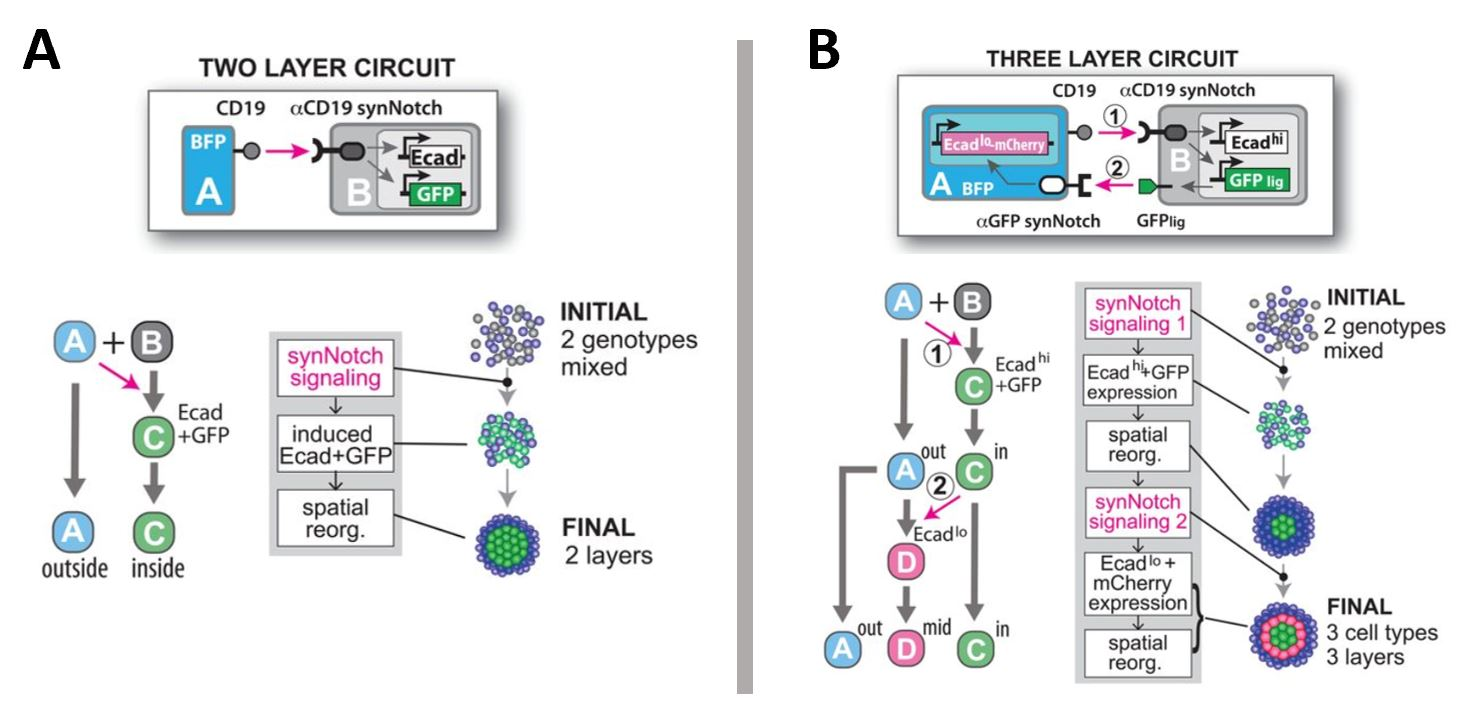
\includegraphics[width=\textwidth]{Todo_etc_al_layer_circuit_design}    % The printed column width is 8.4 cm.
\caption{Todo etc al. Two and Three layer Circuit of Syn- Notch: A) Two layer circuit design from Todo etc al where a mixture of two cell genotypes (A and B) are mixed and Syn-Notch signaling is allowed to occur. A cells activate B cells to turn into green C cells that will express cadherin which leads to agglomeration B) Three layer circuit design from Todo etc al where a mixture of two cell genotypes are mixed and Syn-Notch signaling occurs identical to the two later circuit. A second Syn-Notch pathway is added where activated C cells express Delta 2 which activates Notch 2 on A cells, which leads to the formation of the pink D cell line.  } 
\label{fig:bifurcation}
\end{center}
\end{figure*}

\begin{figure*}
\begin{center}
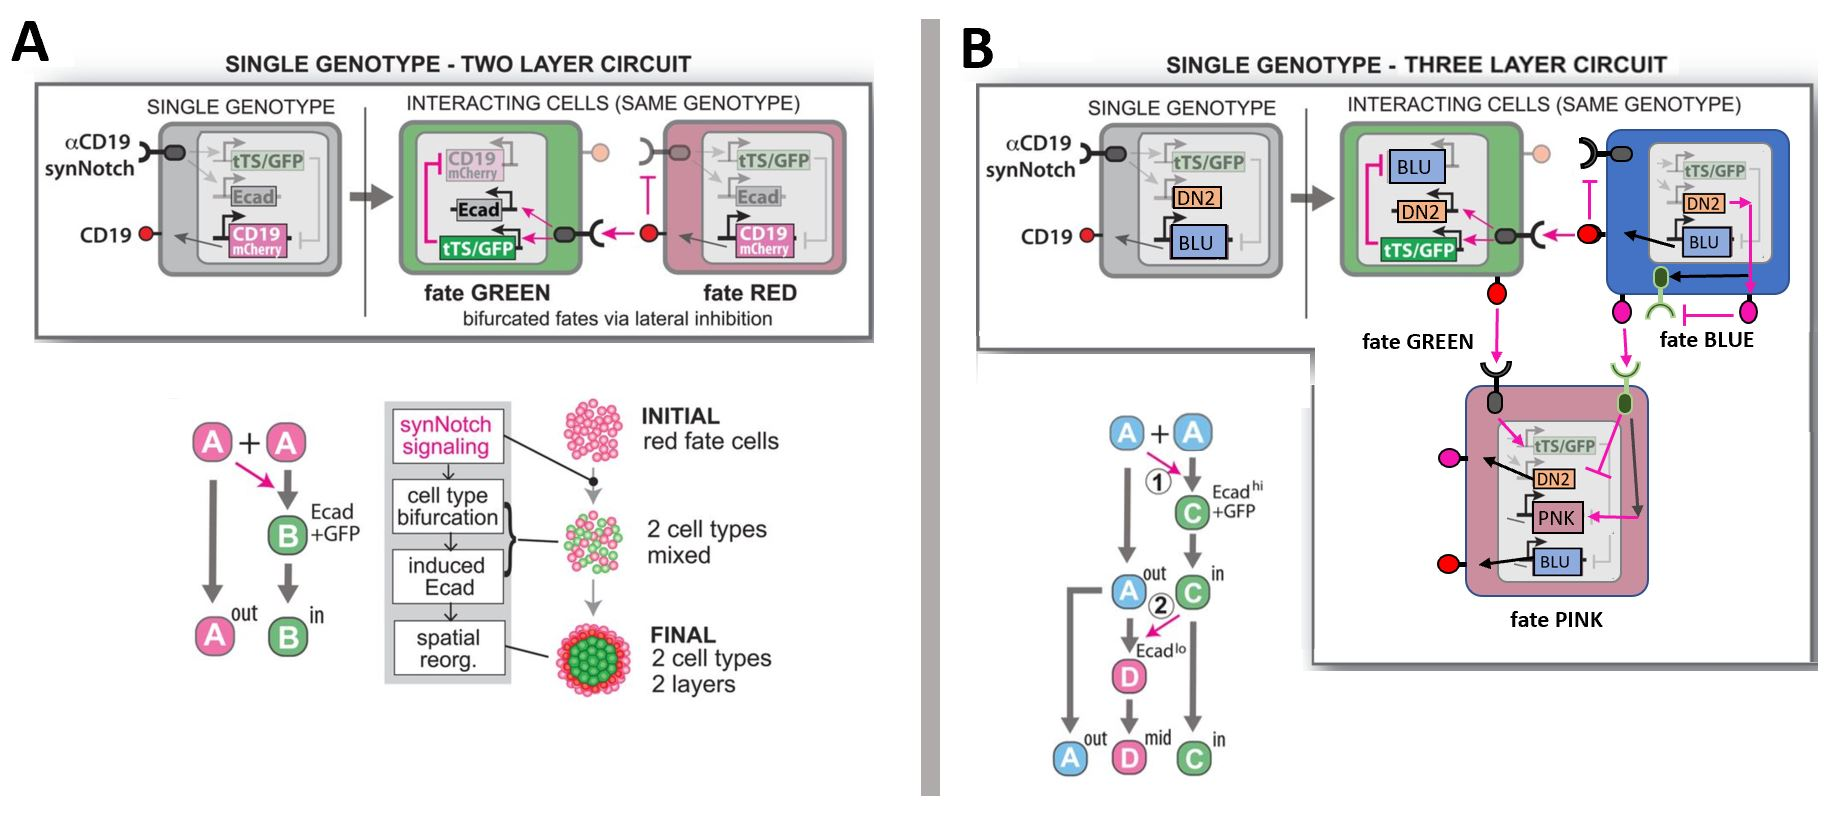
\includegraphics[width=\textwidth]{Modification}    % The printed column width is 8.4 cm.
\caption{Todo etc al. Single Genotype Two layer circuit and Modified Single Genotype Three layer circuit: A) On the left is the original Single Genotype contact inhibition two layer circuit from \cite{TP:18}. Notch and Delta compete and signaling drives the fate of the cell. Notch inhibits the production of Delta and signals green floresence, Delta inhibits on membrane activity of Notch and red floresence is resulted. B) Three layer single genotype Notch-Delta signaling where pink and red Delta and black and green Notch are involved in the signaling. The inhibition and activation is identical to earlier, however only Delta producing cells are blue, Green can produce delta 1, and pink will be completely inhibited and ony Notch 1 and 2 (black and green) are active. } 
\label{fig:bifurcation}
\end{center}
\end{figure*}

\section{Results}

\subsection{Results for Two Genotype -  Two Layer Circuit} 

The Two layer Two genotype circuit operation can be seen in figure 4A. Initially a line of three identical cells are initiated in Netlogo. The Random selection is made, in this case it was set to select one third of the total cells available to be A cells. The A cell produced Delta alone as desired in the circuit and the delta interacted with the Notch on the neighboring black B cell. Cleaved notch (green squares) can be seen accumulating just below the cell membrane of the now green C cell , which became a green cell after enough cleaved notch made it to the nucleus.

Mobility was then added to the cells, specific modifications are further explained according to appendix B to achieve the motion. Cells were initially in the sheet as done before and the staring layout is seen in Appendix B figure 7. Blue A cells and black B cells began moving around Netlogo agent space. As blue A cells reaches a radius close to B cells, the notch pathway activated as desired and many black cells became green B cells. Cadherin was programmed as a binary to save on computer resources, where activation of green fluorescence was also accompanied by cadherin activation. When two green B cells neared each other, and if both expressed Caherin they would slow down compared to other cells, leading to large "masses" of green cells surrounded mostly by individual blue neuron cells not attached to one another. The bias towards the right kept the cells moving, as it was found random direction motion had a tendancy to cause cells to move very little from their staring positions. This likeky due to equal chance it moves anywhere so for every north step there would likely be a south step undoing the progress. 

\subsection{Results for Two Genotype - Three Layer Circuit} 

Three layer was constrained in its geometry, letting two rows of identical cells be generated to resemble a 2 D "Slice" of the balls of cells Todo generated.  Type A cells are again chosen at random, in the case of figure 4B a representative sample was chosen to highlight the proposed slice of the circle of cells. Blue A cells began producing Delta 1 and Notch 2 as desired, where black B cells were only producing Notch 1 as the color indicates. Activation proceeded according to Delta-Notch and the black B cells are now green C cells after an accumulation of Cleaved notch, indicated by the accumulation of cleaved notch just inside the yellow lipid membrane agents. Activation of the second Notch pathway (Delta 2 and Notch 2) is verified by the change of neighboring blue A cells turning pink, indicating the presence of Cleaved notch 2 and further identified by the layer of cleaved Notch 2 (yellow squares) just behind the lipid membrane. The final layout resembles a 2 D slice of a circle of cells taken through the center with a blue exterior and a green interior. This is consistent with \cite{TP:18} visual layers.

\begin{figure*}
\begin{center}
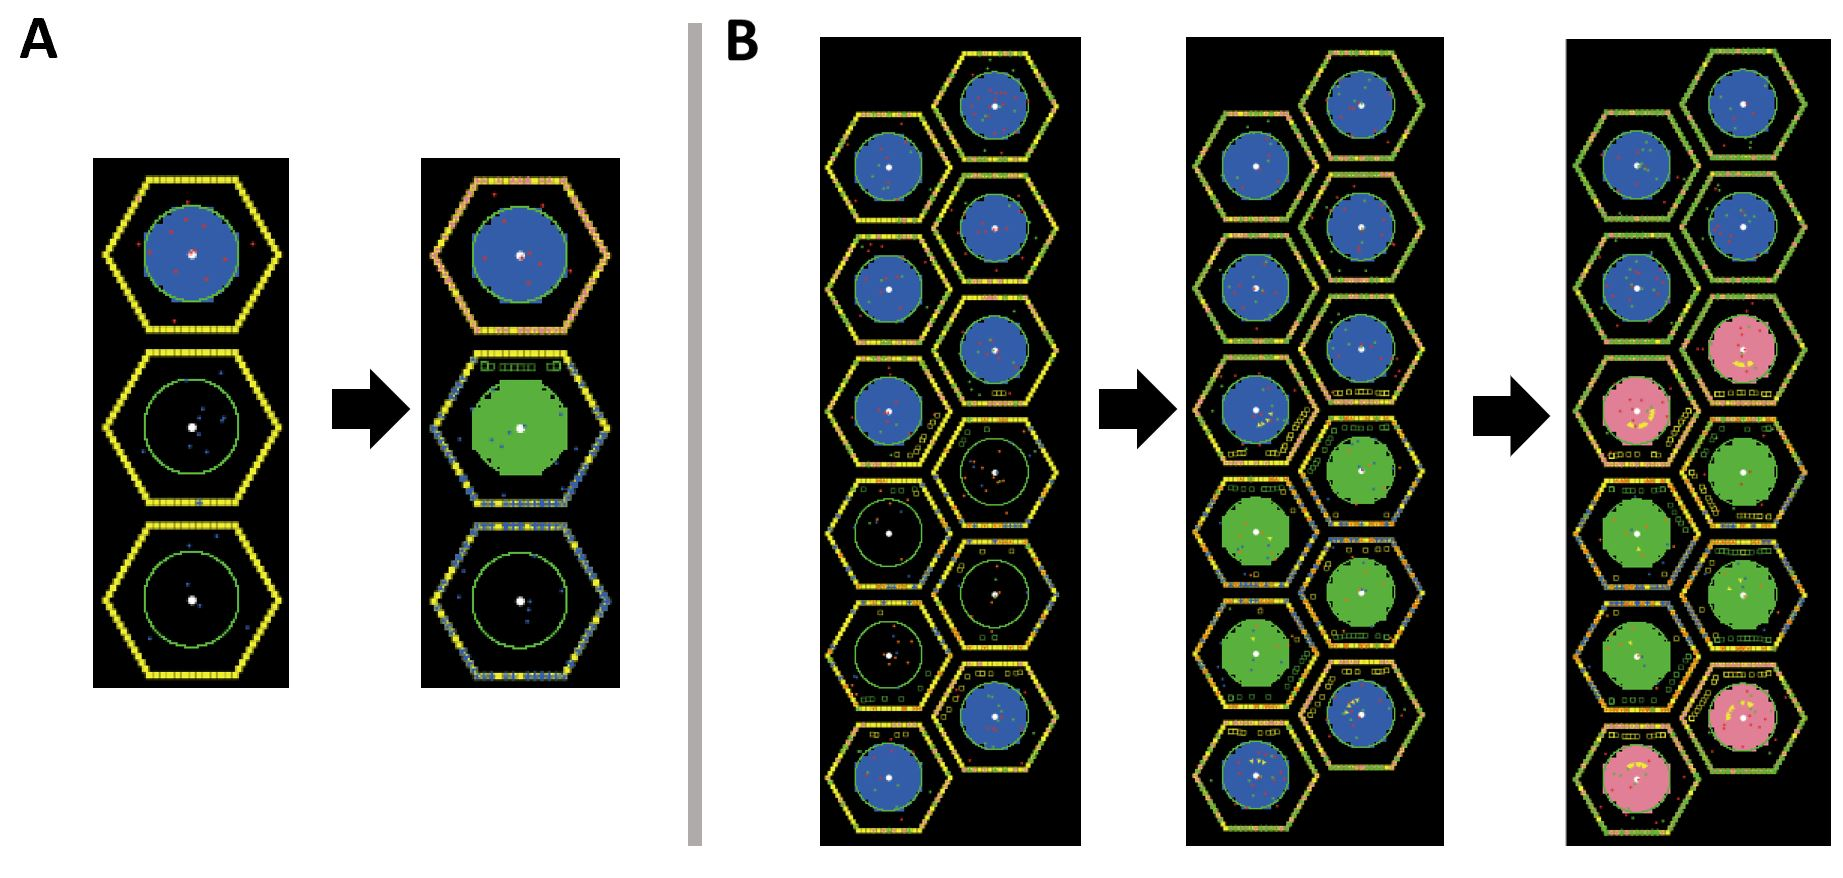
\includegraphics[width=\textwidth]{Two_and_Three_layer_Two_Genotype}    % The printed column width is 8.4 cm.
\caption{Two and Three layer Circuit of Syn- Notch: A) Starting cells are initially allowed to produce either Notch or Delta where Delta producing cells are labeled blue. After time has passed cells expressing Notch have been activated by neighboring blue cells and will turn green. If there are no neighboring cells the Notch expressing cells will remain black. B) Three layer circuit where blue cells are chosen to express Delta and Notch 2. Neighboring cells expressing Notch are activated and turn green and will begin expressing Delta 2. Neighboring blue cells are then activated by green cells' Delta 2 which causes blue cells to turn pink. result is a striped layer structure.  } 
\label{fig:bifurcation}
\end{center}
\end{figure*}

\begin{figure}
\begin{center}
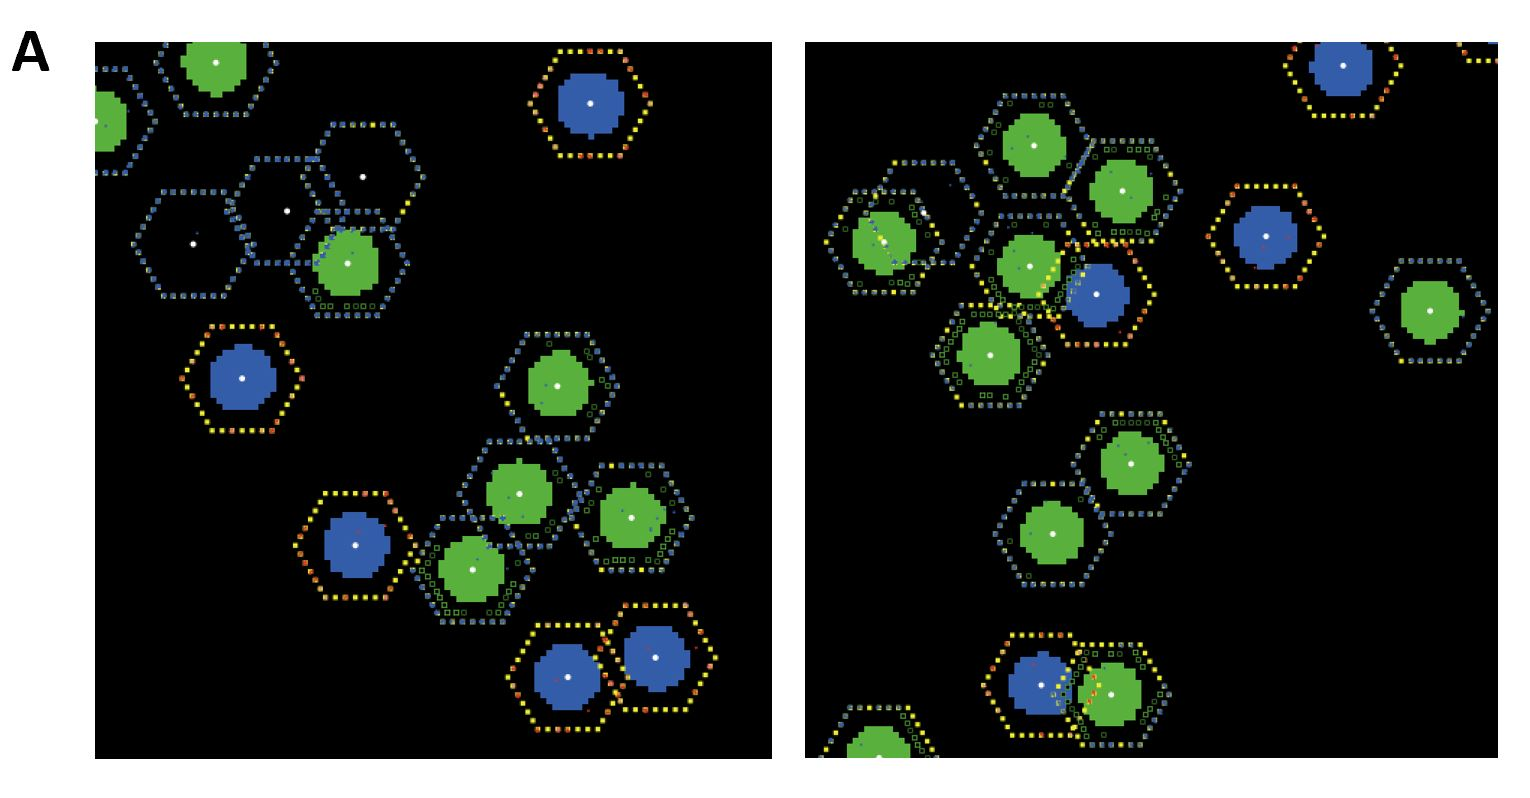
\includegraphics[width=8.0cm]{Mobility_Two_layer}    % The printed column width is 8.4 cm.
\caption{Mobility of Cells in a Two Layer Circuit: A) The addition of the cell mobility into the system introduces the abiltiy of cells to develop the clustering from cadherin expression, Two representative samples are provided. Blue A cells produce Delta which activated black B cells to express cadherin and turn green. When two activated green C cells meet in the agentspace and both are expressing cadherin the speed is reduced "clotting" the green cells. The result is development of green cell clusters and individual blue cells moving arround the clusters. Motion was biased towards the right to allow for adequate mixing of cells.   } 
\label{fig:bifurcation}
\end{center}
\end{figure}


\begin{figure*}
\begin{center}
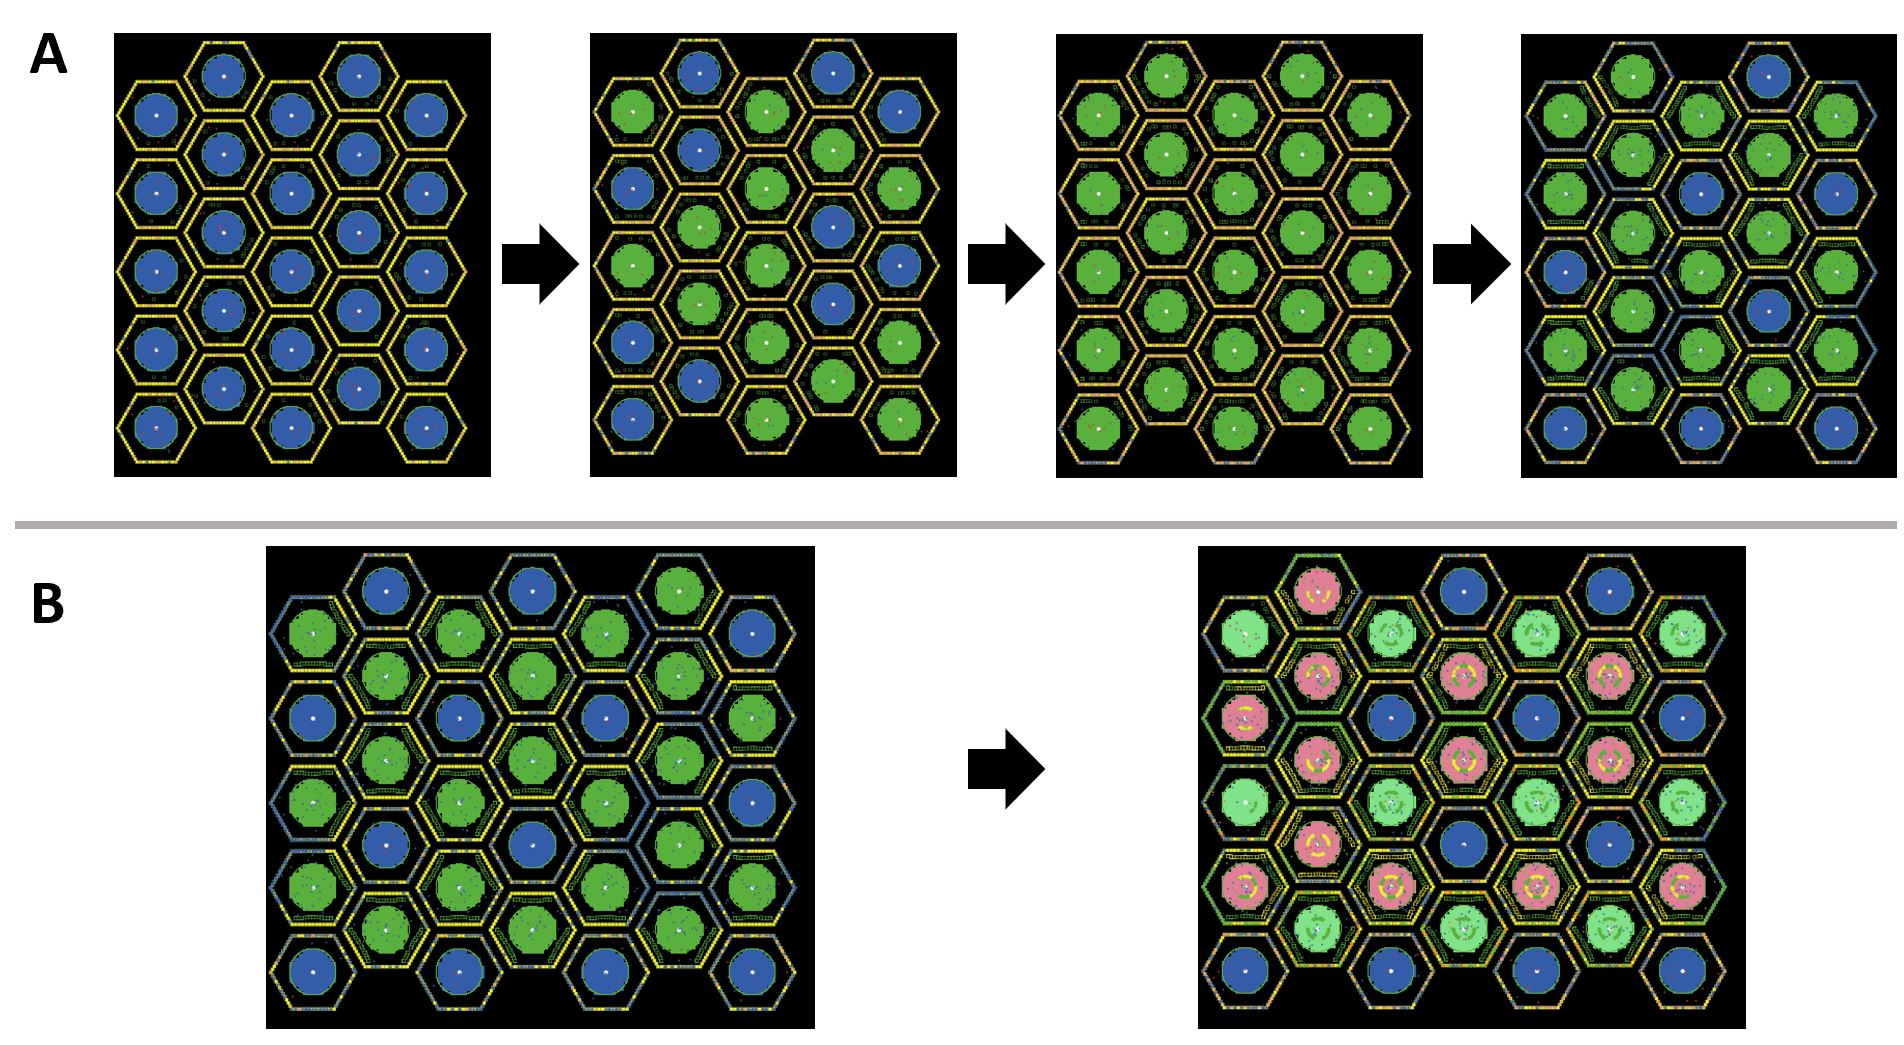
\includegraphics[width=\textwidth]{One_Genotype_two_and_one_SynNotch}    % The printed column width is 8.4 cm.
\caption{Two layer Circuit of Syn- Notch Single Genotype: A) One genotype Delta-Notch signaling replication of \emph{Drosophilla} seen in Reynolds etc al. Cells start of as neurons producing both Notch and Delta, leading to the "tug of war" beteen the cell fates seen as it alternates between all blue and all green cell lines. Eventually an equilibrium is reached which holds the "Rosette" patterns characteristic in \emph{Drosophilla} cell development.  B) The cell sheet on the left is the single Notch-Delta circuit. The right is the change in equilibrium layout after the addition of the second Syn-Notch pathway. Rosettes are now complex combinations of endothelial cells (green and pink) surrounding the central Neuron (blue) cells. } 
\label{fig:bifurcation}
\end{center}
\end{figure*}

\subsection{Results for Single Genotype - Single Notch Two Layer Circuit} 

Results of the single genotype single notch circuit can be put into in the context of both Reynolds \emph{Drosophilla} cells and early random scattering of cells in Todo etc al. The model was able to both verify the "Rosette" pattering seen in Reynolds when signaling was left to reach equilibrium, indicated by an unchaning ammount of blue neurons after a long time. Early patterns before reaching this steady state have features of Todo etc al scattering of cells before cadherin. In figure 6A the formation of the Rosettes occurs only after reaching an equilibrium. Prior to this pattern the cycling between one cell fate and the other, a key feature of Delta-Notch signaling, occurs and matches the initial stages of Todo circuits (second image in A). The pattering is potentially a feature of the geometry of the system and inherent in Notch-Delta signaling, where the additional cadherin component of Toda circuits lead to the loss of Rosettes and formation of the clustering. The results for this model however are limited in the abiltiy to answer that concern where static cells were chosen for single genotype models.

\subsection{Results for Single Genotype - Double Notch Three Layer Circuit} 

To examine if rosette formation could be interrupted by the addition of the second Syn-Notch pathway the model was run and figure 6B shows the new equilibrium state of the three layer circuit. Notable features of the new cell layout is that "Rosette" formation appears to follow a new geometry. Neuron cells, and two types of endothelial cells are present. Neurons are surrounded by both green an pink cell lines in two unique formations. One layout is a blue neuron cell with two pink cells on the left and two on the right with one Green cell above and one green cell below the neuron. The second new layout is the neuron surrounded by green and pink cells, where cells alternate in color as it goes around the neuron. Rosette pattering was retained according to the original definition, in that a single neuron cell is surrounded by cells of endothelial lineage, however the new cell line shows added pattern complexity achived by an additional pathwway. This might be more consistent in actual experiments where cells may rely on more than one pathway to modulate response.





\section{Conclusion}

This paper extended the model developed by Reynolds etc al for \emph{Drosophilla} into proposed circuits developed by Todo etc al for Syn-Notch signaling. Delta-Notch signaling and Todo's Syn-Notch signaling are detailed as a contact signaling pathway present in many cell lines and leads to important developlemtal features of cell growth. Cell patterning was focused on in this series of papers and this paper introduced agent based modeling to further push the modeling efforts to capture the unique pattering that can arise from Delta-Notch and Syn-Notch signaling structures. Removal of signaling capabilities, as was the case in Two and Three layer Two genotype circuits, to allow for directional signaling was able adapt the model to capture key features of Todo etc al experiments. Two layer was able to replicate the singnaling pattern seen by Todo with blue A and green C cell lines bordering each other. Addition of the mobility was able capture the development of the clustering and agglomeration of green C cells that express cadherin. Limitations in the model were unable to capture a large singlular "ball" of cells but instead developed several smaller clusters of cells that still retain organization representative of the larger cluster. Single genotype with both one and two Notch pathways were succesful in replicating Reynolds results in long term equilibrium and early organization held features of Todo scattered patterns. Rosettes were retained when replicating Reynolds results under simmilar parameter setting, however the addion of the second Notch pathway led to complex pattering. The patterns resembled Rosettes however surrounding endothelial cell lines were not limited to a single cell fate, instead multiple unique combinations of the green and pink cell surround the blue neuron cells. Further goals of this work would be to have mobiltiy included in each circuit initially proposed, and not limited to the directional two layer circuit. Limitations of the agent based model are long operating times and poor performance optimization that limited the abiltiy to allow more complicated structures to reach an equilibrium, namely limits imposed on the number of cells was required when mobility was introduced. The advantages the models developed here have is the abiltiy to actively tune parameters and observe the effect on cell patterns, and the ablitiy to represent different circuits instead of just single notch initially developed by Reynolds. The flexibility allows for more complex circuits or simpler circuits to studied in silico, such as the Two Notch single genotype, that may not have been considered in current literature.


\subsection{References and Supporting Information}


\begin{ack}

\textbf{Contribuition and Conception} I want to acknoledge Dr Matthew Paszek and Dr Jefferey Vaner for the project conception and proposal of key directions and goals for the project. I want to further thank them for the feedback provided after the progress report leading to the current paper. I want to thank members of the class for feedback and assistance durring the progress review stage, particularly discussions with Franklin before the presentations about current progress on the modeling and problems we had been running into. \textbf{Data:} Model code will be released on Github via the following link [inset link here]. Four separate models were developed and an example equilibrium state image and the seed that generated the image are also avaliable in the Github and Appendix B supplement of this paper

\end{ack}




\bibliography{Bibliography}             % bib file to produce the bibliography
                                                     % with bibtex (preferred)


\appendix
\section{Modeling}    % Each appendix must have a short title.

Detailed Modeling Descriptions are provided as a PDF of a Readme file from the Github repository. This is attached to the back or provided as a File APPENDIX A.pdf
\section{Supplemental Figures }              % Sections and subsections are supported  

Supplemental Figures are provided in a PDF called SUPPLEMENTAL.pdf and is printed following this page, or if provided elcetronically is labels as SUPPLEMENTAL.pdf
                                                                         % in the appendices.
\end{document}
